\documentclass[uplatex,dvipdfmx]{jlreq}
\usepackage[fleqn,tbtags]{mathtools}
\usepackage{jlreq-deluxe}
\usepackage{geometry}
\usepackage{booktabs}
\usepackage{hyperref}
\usepackage[noalphabet]{pxchfon} % must be after otf package
\usepackage{stix2} %欧文＆数式フォント
\usepackage[fleqn,tbtags]{mathtools} % 数式関連 (w/ amsmath)
\usepackage{url}
\usepackage{here}
\geometry{left=20mm,right=20mm,top=25mm,bottom=25mm}

\title{作業ログ\\ \large プロジェクト名: [加速度センサーを用いた身体動作による輪唱制御システムの構築と視覚フィードバック効果]}
\author{報告者: 早川　和輝}
\date{報告日: 2026年6月10日}

\begin{document}
\maketitle

\section{進捗サマリー(要約)}
\begin{itemize}
    \item 全体進捗率: [50\%]
    \item マイルストーン達成状況: [達成]
    \item 主要成果:
    \begin{itemize}
        \item 成果1: Minimライブラリを利用したアコースティックバイオリンとギロの音色合成プログラムの調整．
        \item 成果2: ArduinoとProcessingの連携の基本的な動作確認．
        \item 成果3: テンポ変更処理の実装の一部．
        \item 成果4: 輪唱の再生の実装の一部．
        \item 成果5: サーボモーターの動作確認．
    \end{itemize}
    \item 重大課題(影響度:無し): なし
\end{itemize}
\section{作業ログ(詳細トラッキング)}
\begin{table}[H]
    \centering
    \small
    \begin{tabular}{lp{1.5cm}p{1.5cm}llp{2.5cm}p{3cm}}
        \toprule
        作業項目 & 開始日 & 完了日 & 状態 & 進捗率 & 依存関係・ブロッカー & コメント \\
        \midrule
        ギロの音色作成& [5/27] & [5/30] & 完了 & 100\% & なし & テンポ重視で作成完了． \\
        ArudinoとProcessingの連携 & [6/3] & [6/8] & 完了 & 100\% & なし & 簡易的に値をarduinoに入れ，Processingで受け取り音楽を流す処理を実装． \\
        音の動作確認 & [6/5] & [6/10] & 進行中 & 100\% & なし & バイオリンとギロの音色の動作確認．音色に問題はなし．\\
        テンポを変更させる処理の追加 & [6/8] & [6/10] & 進行中 & 50\% & なし & テンポ変更の処理の実装の一部．テンポ変更の値を受け取るところまでは完了． \\
        サーボモーターの動作確認 & [6/9] & [6/13] & 進行中 & 50\% & なし & サーボモーターの動作確認． \\
        \bottomrule
    \end{tabular}
\end{table}

\section{担当箇所の計画前のGCと現在のGC}
担当箇所である「楽器演奏実装」における，当初計画時（計画前）のガントチャート（GC）の予定と，現在の進捗・変更状況の比較である．
\begin{table}[H]
    \centering
    \small
    \begin{tabular}{lp{4cm}p{4cm}l}
        \toprule
        タスク名 & 計画前のGC（予定期間） & 現在のGC（実績・修正期間） & 進捗状態 \\
        \midrule
        楽譜作成・Hz出力 & [5/23 $\sim$ 5/25] & [5/23 $\sim$ 5/23] & 完了 \\
        バイオリンの音色作成 & [5/29 $\sim$ 6/6] & [5/25 $\sim$ 5/27] & 完了 \\
        ギロの音色作成 & [5/29 $\sim$ 6/6] & [5/27 $\sim$ 6/6] & 完了 \\
        ArudinoとProcessingの連携 & [6/3 $\sim$ 6/7] & [6/3 $\sim$ 6/7] & 完了 \\
        音の動作確認 & [6/5 $\sim$ 6/9] & [6/5 $\sim$ 6/9] & 完了 \\
        テンポを変更させる処理の追加 & [6/8 $\sim$ 6/13] & [6/8 $\sim$ 6/13] & 着手 \\
        同期との連携 & [6/11 $\sim$ 6/17] & [6/11 $\sim$ 6/17] & 着手 \\
        サーボモーターの動作確認 & [6/9 $\sim$ 6/13] & [6/9 $\sim$ 6/13] & 進行中 \\
        \bottomrule
    \end{tabular}
\end{table}
\begin{figure}[H]
    \centering
    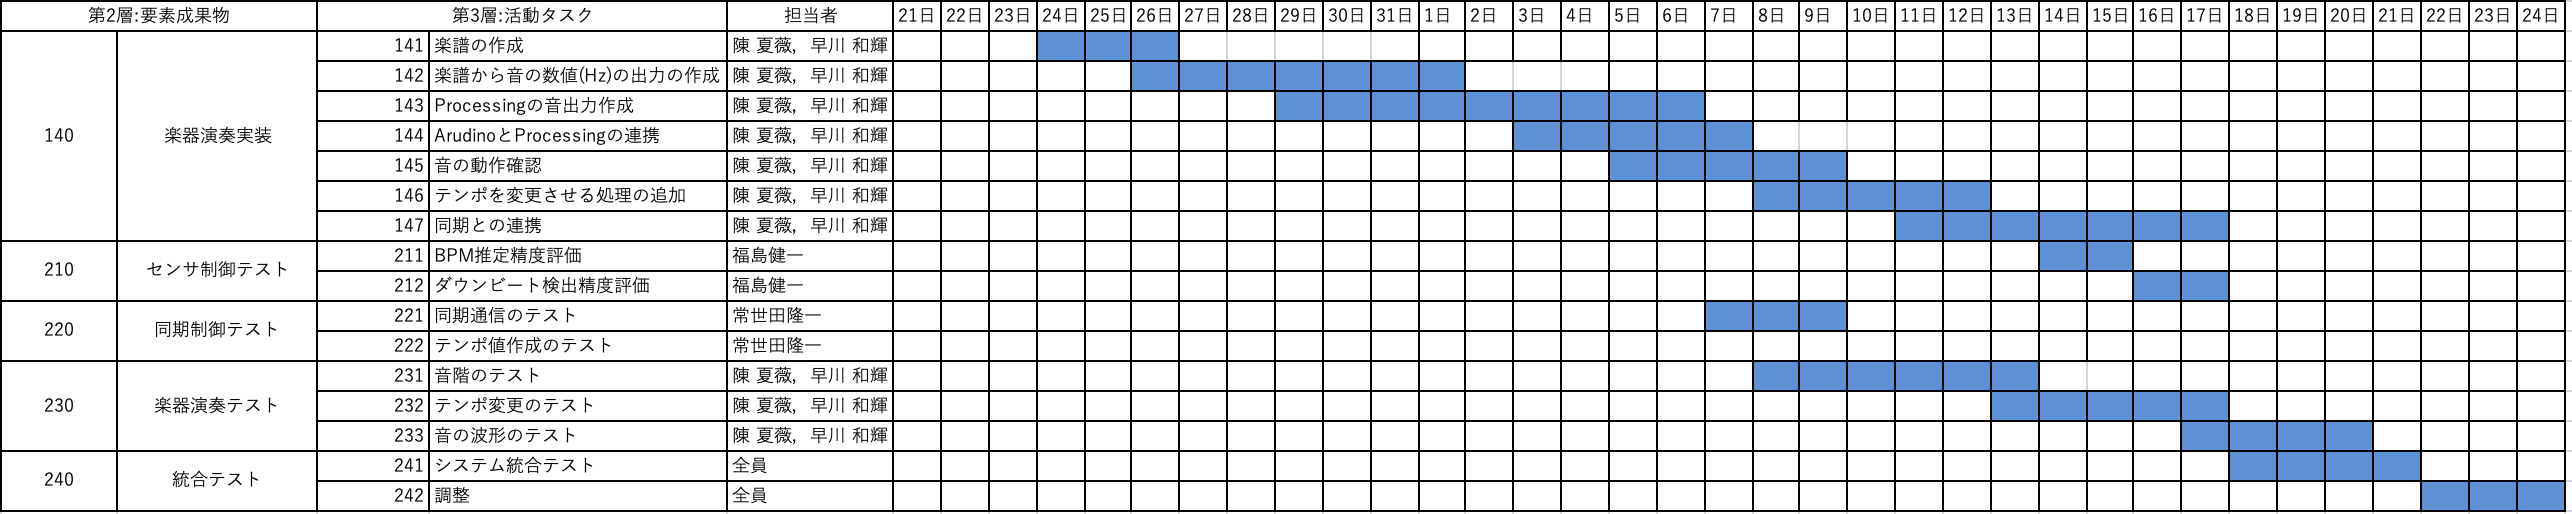
\includegraphics[width=0.8\textwidth]{ganto2.png}
    \caption{ガントチャート}
\end{figure}
\section{日ごとの作業時間と作業内容}
今週実施した日ごとの具体的な作業時間および対応内容の詳細です．
\begin{table}[H]
    \centering
    \small
    \begin{tabular}{lll}
        \toprule
        日付 & 作業時間 & 作業内容 \\
        \midrule
        {}[5/28] & [1.5時間] &ギロの音色の作成．\\
        {}[6/3] & [3.0時間] & ArduinoとProcessingの連携の実装． \\
        {}[6/5] & [1.0時間] & バイオリンとギロの音色の動作確認． \\
        {}[6/8] & [1.5時間] & テンポ変更処理の実装の一部． \\
        {}[6/9] & [1.5時間] & テンポ変更処理の実装の一部． \\
        {}[6/10] & [1.0時間] & テンポ変更処理の実装の一部．全体の動作確認． \\
        \midrule
        \textbf{合計} & \textbf{[9.5時間]} & \\
        \bottomrule
    \end{tabular}
\end{table}
\section{課題管理}
\begin{table}[H]
    \centering
    \small
    \begin{tabular}{p{3cm}p{3cm}llp{3cm}ll}
        \toprule
        課題 & 発生原因 & 影響度 & 優先度 & 対策 & 期限 & 状態 \\
        \midrule
        テンポ変更処理の実装 & テンポ変更の処理が複数のモジュールに関わるため実装が複雑 & 高 & 中 & 処理を段階的に実装し，動作確認をこまめに行う & [6/13] & 進行中 \\
        サーボモーターの動作確認 & サーボモーターの動作確認が不十分 & 中 & 中 & 動作確認を徹底し，問題があれば即座に修正する & [6/13] & 進行中 \\
        同期との連携の実装 & 同期との連携の実装が未着手であるため，今後の作業に影響が出る可能性がある & 中 & 中 & 優先的に着手し，進捗をこまめに報告する & [6/17] & 着手 \\
        \bottomrule
    \end{tabular}
\end{table}
\vspace{0.5em}
\noindent ※影響度=プロジェクトへのインパクト，優先度=対応の緊急性

\section{AI 利用状況と検証(再現性重視)}
\subsection{利用内容}
\begin{itemize}
    \item 利用目的: \LaTeX による作業ログのテンプレート作成
    \item  入力(プロンプト要旨):
    \begin{itemize}
        \item 指定された作業ログのテンプレート項目の生成を依頼 ．
    \end{itemize}
    \item  出力概要:
    \begin{itemize}
        \item テンプレートの構成のコンパイル可能な作業ログの\LaTeX ソースコード ．
    \end{itemize}
\end{itemize}

\subsection{検証方法}
\begin{itemize}
    \item  検証手法: 生成された\LaTeX ソースコードの構造確認およびコンパイル検証
    \item  参照資料: 提供された作業ログテンプレートPDF
    \item  検証手順:
    \begin{enumerate}
        \item 生成されたコードのセクション構成が，テンプレート項目を漏れなく満たしているか目視で確認．
        \item \LaTeX 環境において実際にコンパイルを行い，エラーを吐かずに正しくPDFが生成されるかを確認．
    \end{enumerate}
\end{itemize}

\section{次回計画}
\begin{itemize}
    \item  目標: [同期との連携の実装と，テンポ変更処理の完成]
    \item  達成基準: [同期との連携が実装され，テンポ変更処理が完成すること]
    \item  期限: [6/18]
\end{itemize}

\section{その他}
連絡事項や，他メンバーとの連携が必要な懸念点があれば記載


\end{document}